\documentclass[runningheads]{llncs}
\usepackage{booktabs}
\usepackage{color}
\usepackage{graphicx}
\usepackage{hyperref}

\renewcommand\UrlFont{\color{blue}\rmfamily}

\begin{document}

\title{
    Making History Count
}
\author{Gabriele Cerizza}
\authorrunning{G. Cerizza}

\institute{Università degli Studi di Milano\\
\email{gabriele.cerizza@studenti.unimi.it}\\
\url{https://github.com/gabrielecerizza/information_retrieval_project}}

\maketitle

\section{Introduction}
\label{sec:introduction}

In this report we detail our findings in the study of two tasks related to project number 9 for the Information Retrieval course of University of Milan\footnote{\url{https://island.ricerca.di.unimi.it/\~alfio/shared/inforet/2020-21/inforet-projects.html}}: detection of shifts in the meaning of words across time (Section \ref{sec:semantic_shifts}) and extraction of historical events from text (Section \ref{sec:historical_events}).

\section{Semantic shifts}
\label{sec:semantic_shifts}

The first task is concerned with measuring, in a data-driven way, the diachronic semantic shift or lexical semantic change (LSC) that affected words across time. We proceed to review known approaches to tackle the problem and then we discuss three possible strategies to measure LSC by exploiting word embeddings originated from a corpus of historical documents and from a corpus of contemporary documents.

\subsection{Related work}
\label{subsec:semantic_shifts:related_work}

In literature, the attempts to capture semantic shifts by way of word embeddings can be categorized in mainly two families: static embeddings or type-based models, and contextualized embeddings or token-based models.

\subsubsection{Static embeddings models} Static embeddings represent each word with a single vector. This vector can be considered a summarization of the occurrences of a word in different contexts. Popular static embeddings are obtained from skip-gram with negative sampling (SGNS)~\cite{mikolov-etal-2013-word2vec}, GloVe~\cite{pennington-etal-2014-glove} and fastText~\cite{bojanowski-etal-2017-fasttext}.

Static embeddings can be exploited to detect semantic shifts in a straightforward way. We train two models on corpora of different time periods and then we measure the cosine distance between the embeddings of a given word obtained from the two models~\cite{hamilton-etal-2016-diachronic}. The issue in this direct comparison is that SGNS and the other neural models are stochastic in nature and therefore they produce embeddings that are invariant under rotation. Common solutions include:

\begin{itemize}
    \item orthogonal Procrustes method, which aligns the embeddings to the same coordinate axes~\cite{hamilton-etal-2016-diachronic}, but may introduce noise in the projections~\cite{dubossarsky-etal-2019-time};
    \item initialization of the weights of one model with the weights of the other model, which can be problematic for new words~\cite{kutuzov-etal-2018-diachronic,tahmasebi-etal-2018-survey};
    \item second-order similarity, which compares the cosine similarity of a word to other words in the two models, rather than directly comparing the embeddings of a word~\cite{kutuzov-etal-2018-diachronic,tahmasebi-etal-2018-survey}.   
\end{itemize}

\subsubsection{Contextualized embeddings models} Recently developed neural models like BERT~\cite{devlin-etal-2018-bert} generate different word embeddings for each different context in which a word appears. The pretrained contextualized embeddings are sometimes employed by the authors as is, without fine-tuning on the historical corpus~\cite{rother-etal-2020-cmce,laicher-etal-2021-explaining}. 

Contextualized embeddings models start by extracting a vector for each context, usually a sentence or a portion thereof, in which the word appears in the two corpora. Then, they cluster the vectors of the two periods to find the different senses of a word. After that, they measure how the frequency of the senses changed between the time periods to get an estimate of the semantic shift~\cite{giulianelli-etal-2020-analysing,rother-etal-2020-cmce}. An alternative approach computes the average pairwise distance between each vector of one period and each vector of the other period~\cite{laicher-etal-2021-explaining}.  
 

\subsection{Proposed methods}
\label{subsec:semantic_shifts:methods}

We explored three methods to detect semantic shifts. Two are based on static embeddings and a third one on contextualized embeddings.

\subsubsection{Orthogonal Procrustes method (OP)} We started by collecting pretrained static word embeddings. For the historical corpus we used the embeddings provided in~\cite{sprugnoli-tonelli-2019-histo}. These embeddings were trained with fastText on documents dating from 1860 to 1939 and taken from the Corpus of Historical American English (COHA\footnote{\url{https://corpus.byu.edu/coha/}}) for a total of 198M tokens. For the contemporary corpus we used fastText word embeddings trained on Wikipedia and news\footnote{\url{https://fasttext.cc/docs/en/english-vectors.html}} for a total of 16B tokens and 1M word vectors.

Considering the size of the contemporary vocabulary, as well as the fact that it contained misspelled words, we decided to analyze only the 5000 most frequent words in the contemporary vocabulary, intersected with the historical vocabulary. We also made sure to analyze the “target" words indicated by SemEval-2020~\cite{schlechtweg-etal-2020-semeval} for evaluation purposes (see Subsection~\ref{subsec:semantic_shifts:results}).

Finally, we aligned the vectors with orthogonal Procrustes and computed the cosine distance between the two embeddings of each selected word.

\subsubsection{Nearest neighbors method (NN)} This approach leverages ideas taken from the second-order similarity techniques used with static embeddings. We used the same historical and contemporary word embeddings described for OP. Likewise, we analyzed the same words selected for OP.

The proposed second-order similarity is computed as follows. For each selected word we take the 15 nearest neighbors in the historical vector space; then we measure the cosine distance between the word and these neighbors in the historical vector space; after that, we measure the cosine distance between the word and the same neighbors, but this time in the contemporary vector space; finally we compute the mean squared error (MSE) between the distances measured in the historical vector space and the distances measured in the contemporary vector space. Then we do the same for the 15 nearest neighbors in the contemporary model. Finally, we take the mean between the MSE measured on the historical vector space neighbors and the MSE measured on the contemporary vector space neighbors. 

Given this second-order similarity, we decided to shrink the vocabulary of the two models to their intersection. In this way we guaranteed that each neighbor found in one vector space was also present in the other vector space. 

\subsubsection{Jensen-Shannon distance method (JSD)} This method is based on contextualized embeddings. The corpora were taken from SemEval-2020~\cite{schlechtweg-etal-2020-semeval}. The historical corpus contained shuffled sentences from 1810-1860, while the contemporary corpus contained shuffled sentences from 1960-2010. Both corpora were composed of 6M tokens.

We analyzed the 5000 most frequent words in both corpora, keeping only adjectives, nouns and verbs and filtering stop words, punctuations and tokens containing non-alphabetic characters. We aggregated the embeddings according to lemma and POS tags. Our assumption is that the semantic shift of a word is invariant to declension and conjugation: “cat" and “cats" should be subject to the same semantic shift; likewise for “write" and “wrote". Note that in the previous methods we were not able to distinguish words based on POS, since we only had the embeddings, thus the noun “attack" and the verb “attack" had the same embeddings.

We generated the embeddings from BERT, using the “bert-base-cased"\footnote{\url{https://huggingface.co/bert-base-cased}} pretrained weights, by feeding the transformer with sentences from the corpora. We fine-tuned the model on the historical corpus for 5 epochs. Note that we used only one model to generate embeddings for both time periods. Since BERT generates different embeddings for different contexts, it suffices that BERT acquired knowledge of the contexts used in both time periods~\cite{martinc-etal-2020-leveraging}. For the embeddings, we took only the hidden state of the last layer, which is reportedly the layer most related to semantics~\cite{laicher-etal-2021-explaining}.

Following the approach described in~\cite{rother-etal-2020-cmce}, we first employed an autoencoder to reduce the dimensionality of the embeddings from 768 to 20. Then, the dimensionality was further reduced to 10 with UMAP. The combination of autoencoder and UMAP was shown to be effective for clustering in~\cite{mcconville-etal-2019-n2d}. We clustered the embeddings of a given word with HDBSCAN, which is a variant of DBSCAN with improved robustness and a single hyperparameter~\cite{campello-etal-2013-hdbscan}. 

Interpreting the clusters as senses of a word, we measured the frequency of each sense in the two time periods. Finally, we used the Jensen-Shannon distance to measure the similarity between the two distributions.

\subsection{Results}
\label{subsec:semantic_shifts:results}

In Table~\ref{tab:semantic_shifts:top_words} we show the 10 words whose semantic shift was most prominent according to the proposed methods. In OP we can see many words whose meaning changed due to technological evolution, like “cd", “tv" and “bot". OP and NN also capture shifts of historical or cultural nature, like “isis" and “gay". We observe that the International System of Units was introduced in 1960, hence a possible explanation for the shift in “km". The semantic shifts detected by JSD are not as readily decipherable. 

In Figure~\ref{fig:semantic_shifts:score} we give an example of how the shift in senses was perceived by the JSD method. We can see, for instance, that the verb “score" assumed a meaning more related to sports as the time passed.

\begin{table}
    \caption{Words with the most semantic shift detected by the methods.}
    \label{tab:semantic_shifts:top_words}
    \centering
    \begin{tabular}{lll}
        \toprule
        OP & NN & JSD \\
        \midrule
        cd & deletion & negro (adj.) \\
        romney & km & people (noun) \\
        km & gay & golf (noun) \\
        diff & diff & shopping (noun)  \\
        deletion & outstanding & overall (adj.) \\
        tv & implement & businessman (noun) \\
        template & highlight & switch (verb) \\
        isis & parameter & investor (noun) \\
        bot & red & motor (noun) \\
        highlight & template & user (noun) \\
        \bottomrule
    \end{tabular}
\end{table}

\begin{figure}
    \center
    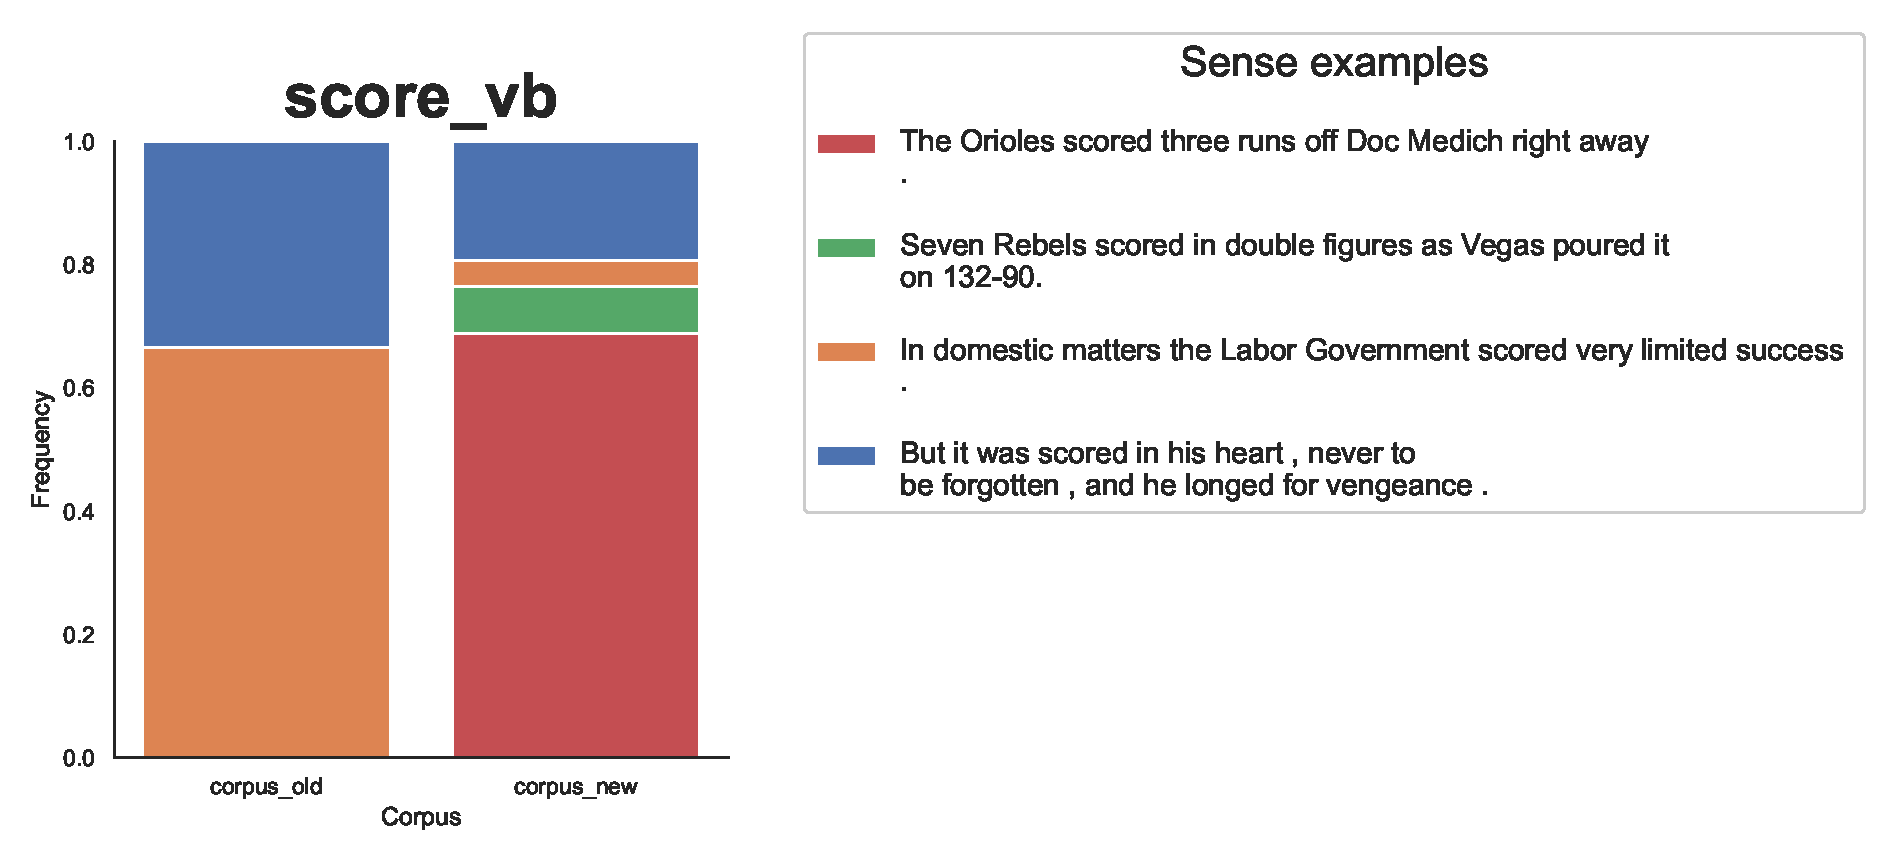
\includegraphics[width=0.7\textwidth]{img/33_score_vb.eps}
    \caption{Shift in the frequency of senses for the verb “score".} 
    \label{fig:semantic_shifts:score}
\end{figure}

The instructions provided for project number 9 state that the evaluation of the results will be carried out by experts in the linguistics and history domains. To this end, detailed results for each method can be perused in our repository.

Furthermore, we evaluated our results against a ground truth for the semantic shift occurred in 37 words provided by SemEval-2020~\cite{schlechtweg-etal-2020-semeval}. In Table~\ref{tab:semantic_shifts:spearman} we compare the Spearman's rank-order correlation of our methods with the 5 top systems in the SemEval-2020 shared task. We deduce that our methods are competitive with other state-of-the-art systems.

\begin{table}
    \caption{Spearman's rank-order correlation to SemEval-2020 ground truth for the proposed methods and the top systems in the competition.}
    \label{tab:semantic_shifts:spearman}
    \centering
    \begin{tabular}{|c|c|c|c|c|c|c|c|}
        \toprule
        OP & NN & JSD & UG\_Student\_Intern & Jiaxin \& Jinan & cs2020 & UWB & Discovery\_Team \\
        \midrule
        .391 & .341 & .365 & .422 & .325 & .375 & .367 & .361 \\
        \bottomrule
    \end{tabular}
\end{table}

\subsection{Conclusion}
\label{subsec:semantic_shifts:conclusion}

Tables~\ref{tab:semantic_shifts:top_words} and~\ref{tab:semantic_shifts:spearman} suggest that, on the LSC task, static embeddings methods perform slightly better than contextualized embeddings methods. The same conclusion can be found in literature~\cite{laicher-etal-2021-explaining,schlechtweg-etal-2020-semeval}. Possible reasons for this behavior are the small size of the corpora for the JSD method and a need of further fine-tuning. Another possible reason is the fact that the historical corpus contains a lot of artifacts and wrongly tokenized words.

Apart from these issues, a possible improvement in the JSD method involves tuning the HDBSCAN hyperparameter to find a number of senses for each word that is similar to the number of word synsets found in WordNet.

\section{Historical events extraction}
\label{sec:historical_events}

\bibliographystyle{splncs04}
\bibliography{bibtex_entries}

\end{document}